\def\iStart{0} \def\iEnd{7}
\def\jStart{0} \def\jEnd{7}
\def\kStart{0} \def\kEnd{7}

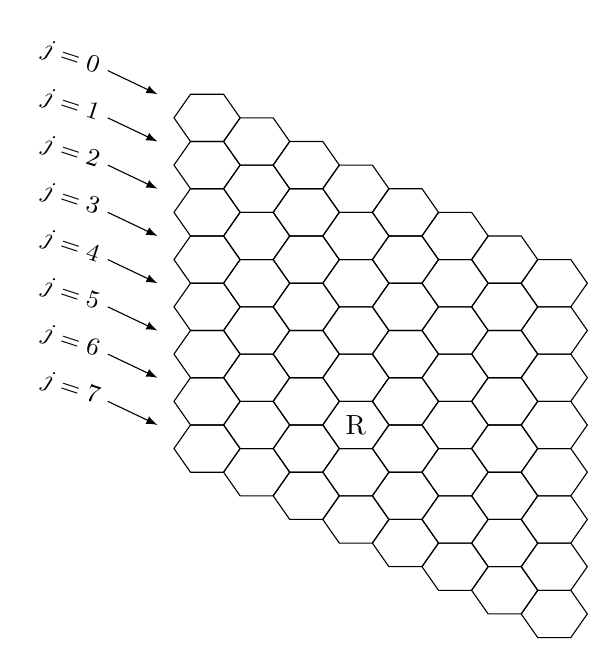
\begin{tikzpicture}[scale=.3, xscale=.7, yscale=-1]
  % --
  \foreach\i in {\iStart, ..., \iEnd} {
    \foreach\j in {\jStart, ..., \jEnd} {
      \edef\x{3 * \i}
      \edef\y{2 * \j + \i}
      \draw (\x - 1, \y - 1) -- ++( 2,  0) -- ++( 1,  1) --
          ++(-1,  1) -- ++(-2,  0) -- ++(-1, -1) -- cycle;
    }
  }

  \foreach\j in {\jStart, ..., \jEnd} {
    \edef\x{-3}
    \edef\y{2 * \j - 1}
    \node[anchor=east, rotate=-18, font=\small] at (\x - 3, \y - 1) {\(j = \j\)};
    \draw[-latex] (\x - 3, \y - 1) -- (\x, \y);
  }

  \def\i{3}\edef\x{3 * \i}
  \def\j{5}\edef\y{2 * \j + \i}

  \node at (\x, \y) {R};

\end{tikzpicture}
